\documentclass[11pt,a4paper]{article}
\usepackage[margin=21mm]{geometry}
\usepackage{fontspec}\setmainfont{Times New Roman}
\usepackage{amsmath,amssymb,mathtools,booktabs,array,tabularx,xcolor,fancyhdr,microtype,graphicx,enumitem}
\usepackage[hidelinks]{hyperref}
\definecolor{ink}{HTML}{16324F}
\pagestyle{fancy}\fancyhf{}\fancyhead[L]{\small\textcolor{ink}{QEF-QIRBP v2: corrected implementation and security analysis}}
\fancyhead[R]{\small 19 October 2026}\fancyfoot[C]{\thepage}
\setlength{\headheight}{14pt}\setlength{\parindent}{0pt}\setlength{\parskip}{6pt}
\setlist{nosep,leftmargin=*}
\newcommand{\ket}[1]{|#1\rangle}\newcommand{\bra}[1]{\langle#1|}
\newcommand{\E}{\mathbb E}\newcommand{\Id}{\mathbb I}
\newcommand{\tr}{\operatorname{Tr}}\newcommand{\xor}{\mathbin{\oplus}}
\newcommand{\Rtau}{\mathcal R_\tau}
\newcolumntype{Y}{>{\raggedright\arraybackslash}X}
\begin{document}
\begin{center}
{\LARGE\bfseries\textcolor{ink}{QEF-QIRBP v2}}\\[4pt]
{\large Corrected unitary implementation, exact privacy theorem,}\\
{\large and complete results on the four original images}\\[4pt]
{\small Native resolutions and \(256\times256\); three fresh keys per case}
\end{center}
\section*{1. The final resistance formula}
For the repaired variant defined in this report, let \(N\) be the number of valid pixel addresses, \(n=\lceil\log_2N\rceil\), \(r=11\), and \(D=N2^r\). The public dimensions are fixed in each security game. Under the specified independent uniform privacy-key model,
\[
\boxed{
(\mathcal E\otimes\Id_R)(\rho_{PR})
=\frac{\Id_{\rm valid}}{D}\otimes\rho_R
\quad\text{for every valid joint input }\rho_{PR}.
}
\]
The reference register \(R\) may contain arbitrary adversarial side information about the input, independent of the secret key source. Therefore
\[
\boxed{
\epsilon_{\rm priv}:=\tfrac12\|\mathcal E-\Rtau\|_\diamond=0,\quad
P_{\rm guess}^{\rm opt}=\tfrac12,\quad
\operatorname{Adv}_{\rm excess}^{\rm fresh}(q)=0.
}
\]
The diamond norm is over the valid input subspace, including reference systems; \(\Rtau(X)=\tr(X)\Id_{\rm valid}/D\). Every oracle call and every physical ciphertext preparation uses a fresh independent key. These are exact mathematical values in the stated model, not fitted image-quality scores.

\textbf{Material correction.} This result concerns the implemented v2 variant. Its uniform amplitude/phase masks and unbiased secret offset are new, explicit key-law requirements. The reference provider uses Python \texttt{secrets} OS randomness \cite{secrets}; the per-pixel mixing angles use SHAKE. No nD-HCS or HG\(\Phi\)-QRNG output distribution, physical QRNG certification, or IBM hardware execution is claimed here.

\textbf{Completed experiments.} All 24 complete image encryptions/decryptions recovered the original RGB bytes exactly. Independent dense matrices, exhaustive small-key channels, phase-key diagnostics, and privacy-core ablations corroborate the implementation. The following pages give every table and the derivation.

\begin{center}
{\small
\setlength{\tabcolsep}{4pt}
\begin{tabular}{@{}lrrrr@{}}
\toprule
Native image & $N$ & $Q$ & Exact recoveries & Ideal $\epsilon_{\rm priv}$ \\
\midrule
IM1 & 65,536 & 27 & 3/3 & 0 \\
IM2 & 50,394 & 27 & 3/3 & 0 \\
IM3 & 65,536 & 27 & 3/3 & 0 \\
IM4 & 786,432 & 31 & 3/3 & 0 \\
\bottomrule
\end{tabular}}
\end{center}


The public ciphertext in the theorem is a quantum state. PNG previews and optional full-amplitude simulator checkpoints are diagnostic classical descriptions, outside that security target.

\newpage
\section*{2. Exact encoding, key layout, and repaired layers}
\textbf{Encoding.} For each pixel \(k\), plane \(\ell\in\{0,\ldots,7\}\), and wavelength label \(\lambda\in\{0,\ldots,31\}\), let \(d_{k,\ell}\) be the three RGB bits. The source images have no wavelength-dependent extra measurements:
\[
\ket{I}=\frac1{\sqrt{256N}}\sum_{k,\ell,\lambda}
 \ket{k}\ket{d_{k,\ell}}\ket{\ell}\ket{\lambda}.
\]
There are \(256N\) orthogonal terms, so this state has norm one. The feature register has \(3+3+5=11\) qubits. The five wavelength qubits are replicated labels, not additional spectral measurements.

\textbf{Key fields.} The private key record stores three 128-bit fields \(A,P,B\), totalling 384 storage bits. From \(A\), reserve independent uniform
\[
z\in\{0,1\}^n,\qquad u,v\in\{0,1\}^r.
\]
The remaining \(128-n-2r\) bits seed the per-pixel Euler mixing \(W_k\), independently of these reserved bits:
\[
W_k=\bigotimes_{j=1}^r R_z(\theta^z_{k,j})R_y(\theta^y_{k,j})R_x(\theta^x_{k,j}).
\]
SHAKE deterministically supplies the diagnostic mixing angles in this implementation. The proof permits any unitary \(W_k\) independent of the reserved bits.

\textbf{Substitution.} With
\[
V_{u,v}=\bigotimes_j R_z(\pi v_j)R_x(\pi u_j),
\quad
R_k=(-1)^{z\cdot k}V_{u,v}W_k,
\quad
R_{\rm sub}=\sum_k\ket k\bra k\otimes R_k,
\]
the uniform Pauli mask and relative position phases are inside the same substitution macro layer. The sign is a relative phase across positions. It may be implemented by position \(Z\) gates or by a controlled \(2\pi\) feature rotation.

\textbf{Permutation.} Split \(P\) into independent 64-bit words. The first selects a coefficient \(a\) coprime to \(N\). Rejection-sample the second word \(w\) until
\[
0\le w<L,\qquad L=\lfloor2^{64}/N\rfloor N,
\qquad s=w\bmod N .
\]
Then \(s\) is exactly uniform on \(\{0,\ldots,N-1\}\), independently of \(a\). Set
\[
\pi_{a,s}(k)=(ak+s)\bmod N,\qquad
\pi_{a,s}^{-1}(t)=a^{-1}(t-s)\bmod N.
\]
Invalid padded addresses are extended by the identity. The accepted key domain has size \(2^{320}L\); 384 is its record length, not a proved search-security exponent.

\textbf{Entanglement.} The field \(B\) chooses position-controlled CNOT/CZ gates in an explicit chronological order. Thus \(E_B=\sum_t\ket t\bra t\otimes T_B(t)\). Its aggregate Pauli implementation retains every commutation phase and is checked against dense chronological gates.

\newpage
\section*{3. Correctness and privacy: the complete derivation}
For fixed key values,
\[
U_K=E_BP_{\pi_{a,s}}R_{\rm sub},\qquad
U_K^\dagger=R_{\rm sub}^\dagger P_{\pi_{a,s}}^\dagger E_B^\dagger .
\]
Each block \(R_k\), each permutation, and each CNOT/CZ is unitary. Orthogonal position projectors give
\[
R_{\rm sub}^\dagger R_{\rm sub}=\Id.
\]
Consequently \(U_K^\dagger U_K=\Id\), proving exact decryption.

For secrecy, condition on the remaining mixing seed, \(a\), and \(B\). They can be arbitrary: their secrecy or randomness is not needed below. Expand an arbitrary valid plaintext/reference state as
\[
\rho_{PR}=\sum_{k,l=0}^{N-1}\ket k\bra l\otimes X_{kl},
\]
where \(X_{kl}\) acts on the feature and reference registers.

First, average the uniform phase mask. Binary-character orthogonality gives
\[
2^{-n}\sum_z(-1)^{z\cdot(k\xor l)}=\delta_{kl}.
\]
This removes all off-diagonal position blocks, including for \(N<2^n\). Second, uniform feature Pauli twirling yields
\[
\E_{u,v}[(V_{u,v}\otimes\Id_R)Y(V_{u,v}^\dagger\otimes\Id_R)]
=\Id_{2^r}/2^r\otimes\tr_{\rm feat}(Y).
\]
Partial trace is invariant under each \(W_k\), so after substitution averaging the state is
\[
\sum_k\ket k\bra k\otimes\frac{\Id_{2^r}}{2^r}\otimes\tr_{\rm feat}(X_{kk}).
\]
The permutation moves \(k\) to \(ak+s\bmod N\). Position-controlled \(E_B\) leaves every maximally mixed feature block unchanged. Finally, for each fixed \(k,a\), uniform \(s\) sends \(k\) uniformly to every valid output address:
\begin{align*}
(\mathcal E\otimes\Id_R)(\rho_{PR})
&=\frac1N\sum_t\ket t\bra t\otimes\frac{\Id_{2^r}}{2^r}
  \otimes\sum_k\tr_{\rm feat}(X_{kk})\\
&=\frac{\Id_{\rm valid}}{N2^r}\otimes\rho_R .
\end{align*}
This proves the boxed formula on page 1 for every valid input, including entangled references.

The mechanism is a private-quantum-channel randomization, related to quantum one-time-pad results \cite{private}; it is not claimed as a newly discovered cryptographic primitive. Per-pixel mixing and the entangling layer can coexist with this proof, but sensitivity or chaos is not substituted for the twirling identities.

\newpage
\section*{4. Imperfect keys, attack models, and limits}
Let \(\zeta=(z,u,v,s)\) be the privacy core. Let \(\eta\) contain the remaining mixing and gate-selection material. If its real joint key/adversary state is within trace distance
\[
\Delta=\tfrac12\|\rho_{\zeta E\eta}
 -(U_\zeta\otimes\rho_{E\eta})\|_1
\]
of the ideal independent uniform core, contractivity gives the general formula
\[
\boxed{\epsilon_{\rm priv}\le\Delta,\qquad
\operatorname{Adv}_{\rm excess}^{\rm fresh}(q)
\le\min\{\tfrac12,q\Delta\}.}
\]
For entirely classical information, this is total variation distance. The implementation's exact rejection rule and disjoint bit allocation give \(\Delta=0\) in the trusted uniform-bit model. Image histograms cannot certify a physical source's \(\Delta\).
For the \(q\)-call bound, the same conditional guarantee is required at each call, with \(E\) including previous adversarial history.

\begin{tabularx}{\linewidth}{@{}p{34mm}Y@{}}
\toprule
Attack or property&Correct statement for this implementation\\
\midrule
Ciphertext-only discrimination&Zero ideal advantage, including all quantum POVMs.\\[4pt]
Known pairs under other fresh keys&No added information about the challenge plaintext from the ciphertext channel.\\[4pt]
Fresh-key chosen-plaintext calls&Zero ideal advantage for \(q\) valid-input calls; the reference-system proof includes adaptive quantum memory.\\[4pt]
Independent encryptions of one image&The joint ciphertext is \(\tau^{\otimes q}\), independent of the image. Tomography estimates the averaged state, not a shared-key pure ciphertext.\\[4pt]
Fixed-key oracle or repeated copies&Outside this one-use protocol. Reusing one key invalidates the independent-channel argument.\\[4pt]
Generic Grover key search&A nominal \(O(2^{192})\) search estimate is not an attack lower bound or the privacy proof. No such exponent is asserted.\\[4pt]
Authentication / tamper detection&Not supplied by these unitary layers. An authentication code would be an additional mechanism.\\[4pt]
PNG or full-state description&Not the quantum ciphertext target. No classical-file secrecy claim is made for diagnostic previews or simulator checkpoints.\\
\bottomrule
\end{tabularx}

The scope is public fixed dimensions and valid address support. A single unknown quantum ciphertext state is not equivalent to providing its complete classical amplitude description. Every physical ciphertext preparation, including another preparation of the same image, requires a new independent key.

\newpage
\section*{5. Inputs, repetitions, and computational method}
The four original source images were copied without changing their source bytes. IM1 uses the colour source loaded by the original driver. That source is \path{Ashurbanipal.jpg}, distinct from the separately exported grayscale preview. The native profile retains the actual source dimensions.

\begin{center}
{\small
\setlength{\tabcolsep}{4pt}
\begin{tabular}{@{}llrr@{}}
\toprule
Image & Source file & Width $\times$ height & Pixels $N$ \\
\midrule
IM1 & IM1\_Ashurbanipal.jpg & $256\times256$ & 65,536 \\
IM2 & IM2\_IM2\_original.png & $227\times222$ & 50,394 \\
IM3 & IM3\_IM3\_original.png & $256\times256$ & 65,536 \\
IM4 & IM4\_IM4\_original.jpg & $1024\times768$ & 786,432 \\
\bottomrule
\end{tabular}}
\end{center}


A second profile uses the same source images resized to \(256\times256\) with Pillow LANCZOS. It is explicitly distinguished from native-resolution tests. Each profile/image uses three fresh independently sampled key records: \(4\times2\times3=24\) complete runs.

\textbf{Exact factorized simulation.} For each position, the RGB/plane subsystem has 64 complex amplitudes and the five wavelength qubits have five two-component factors. Because the input's wavelength labels contain no additional spectral dependence, and every per-position operation is a product of one-qubit rotations or Paulis, this representation is exact. It preserves coherent phases between positions and does not measure at chunk boundaries.

Batches of 2,048 positions keep memory bounded without changing the unitary map. Full dense storage would require \(16\cdot2^Q\) bytes for complex128, including 32 GiB at \(Q=31\). The large-image computation instead processes exact conditional branches.

\textbf{Independent checks.} The production representation was compared with dense matrices assembled independently from tensor-product rotations, address permutations, and chronological CNOT/CZ basis actions. Matrix tests include a non-power-of-two pixel count. The local 7-by-7 SSIM calculation was independently checked against direct window calculations.

These are local classical simulator results. No IBM hardware, noisy-device fidelity, or physical random-source experiment was executed. Original experiment files and source-image files remained unchanged; their integrity checks are included in the results.

\newpage
\section*{6. Complete image recovery}
Every row below aggregates three independently keyed complete runs. All reconstructed images match the source profile's RGB bytes. PSNR is infinite because MSE is exactly zero; SSIM uses 7-by-7 windows.

\begin{center}
{\small
\setlength{\tabcolsep}{4pt}
\begin{tabular}{@{}lrrrrrr@{}}
\toprule
Profile/image & Exact & MSE & SSIM & PSNR & Max $|1-F|$ & Max norm error \\
\midrule
Native/IM1 & 3/3 & 0 & 1 & $\infty$ & $1.55\times10^{-15}$ & $3.77\times10^{-15}$ \\
Native/IM2 & 3/3 & 0 & 1 & $\infty$ & $2.00\times10^{-15}$ & $4.11\times10^{-15}$ \\
Native/IM3 & 3/3 & 0 & 1 & $\infty$ & $1.55\times10^{-15}$ & $4.22\times10^{-15}$ \\
Native/IM4 & 3/3 & 0 & 1 & $\infty$ & $4.44\times10^{-16}$ & $4.00\times10^{-15}$ \\
256/IM1 & 3/3 & 0 & 1 & $\infty$ & $1.55\times10^{-15}$ & $3.89\times10^{-15}$ \\
256/IM2 & 3/3 & 0 & 1 & $\infty$ & $1.55\times10^{-15}$ & $3.89\times10^{-15}$ \\
256/IM3 & 3/3 & 0 & 1 & $\infty$ & $1.55\times10^{-15}$ & $3.77\times10^{-15}$ \\
256/IM4 & 3/3 & 0 & 1 & $\infty$ & $1.33\times10^{-15}$ & $3.89\times10^{-15}$ \\
\bottomrule
\end{tabular}}
\end{center}


The fidelity is computed from the coherent global overlap, not from the mean of per-pixel fidelities:
\[
F=\left|\frac1N\sum_k
 \langle\chi_k|\chi_k^{\rm recovered}\rangle\right|^2.
\]
Wavelength tensor-factor phases are handled with a compensating core phase, preserving the full state exactly. Numerical roundoff is reported separately from the ideal security theorem.

\begin{center}
{\small
\setlength{\tabcolsep}{4pt}
\begin{tabular}{@{}ll@{}}
\toprule
Check & Observed result \\
\midrule
Complete runs & 24/24 \\
Original source bytes unchanged & Yes \\
Recovered RGB bytes identical & All 24 runs \\
Largest recovered amplitude error & $7.26\times10^{-16}$ \\
Independent SSIM-window error & $9.71\times10^{-17}$ \\
\bottomrule
\end{tabular}}
\end{center}


The complete per-run values, byte hashes, local simulator timings, and inspection metrics are in the CSV file:
\begin{quote}\texttt{results/all\_runs.csv}\end{quote}
Saved decrypted PNGs use the first key of each profile/image; all three keys were verified over the entire image.
Checking every recovered RGB byte here uses simulator access to the recovered amplitudes. It does not claim full classical-image extraction from one physical quantum state. Physical image readout requires repeated preparations and measurements, with a fresh key on every ciphertext preparation.

\newpage
\section*{7. Exhaustive channel, dense operator, and ablation results}
For small valid dimensions, every privacy-core key and every offset was enumerated, conditional on fixed mixing/gate material. The normalized Choi matrix was compared with \(I_{D^2}/D^2\). A random entangled reference was independently tested. These are numerical corroborations; the exact theorem covers all dimensions.

\begin{center}
{\footnotesize
\setlength{\tabcolsep}{4pt}
\begin{tabular}{@{}lrrrrrr@{}}
\toprule
$N$ & $r$ & $D$ & Keys & Choi trace distance & Reference distance & $P_{\rm guess}$ \\
\midrule
2 & 1 & 4 & 16 & $1.01\times10^{-16}$ & $1.18\times10^{-16}$ & 0.500000000000 \\
3 & 1 & 6 & 48 & $1.98\times10^{-16}$ & $1.61\times10^{-16}$ & 0.500000000000 \\
4 & 1 & 8 & 64 & $1.26\times10^{-16}$ & $1.63\times10^{-16}$ & 0.500000000000 \\
2 & 2 & 8 & 64 & $1.02\times10^{-16}$ & $1.28\times10^{-16}$ & 0.500000000000 \\
3 & 2 & 12 & 192 & $2.00\times10^{-16}$ & $1.20\times10^{-16}$ & 0.500000000000 \\
4 & 2 & 16 & 256 & $1.41\times10^{-16}$ & $6.77\times10^{-16}$ & 0.500000000000 \\
\bottomrule
\end{tabular}}
\end{center}


The Choi trace distance is a diagnostic, not silently equated to diamond distance. The exact algebra proves diamond-distance zero in the ideal model. Observed residuals reflect floating-point arithmetic.

\begin{center}
{\footnotesize
\setlength{\tabcolsep}{4pt}
\begin{tabular}{@{}lrrrrr@{}}
\toprule
$N$ & $r$ & $D$ & Unitarity error & Dense/output error & Recovery $L_2$ error \\
\midrule
4 & 7 & 512 & $1.33\times10^{-15}$ & $4.73\times10^{-17}$ & $4.27\times10^{-16}$ \\
4 & 7 & 512 & $8.88\times10^{-16}$ & $6.21\times10^{-17}$ & $3.61\times10^{-16}$ \\
3 & 6 & 192 & $8.88\times10^{-16}$ & $5.93\times10^{-17}$ & $4.74\times10^{-16}$ \\
3 & 6 & 192 & $8.88\times10^{-16}$ & $5.00\times10^{-17}$ & $4.06\times10^{-16}$ \\
\bottomrule
\end{tabular}}
\end{center}


\textbf{Ablations.} Removing the position phases, the feature masks, or the exactly uniform offset breaks the complete valid-input privacy channel in the tested example:
\begin{center}
{\small
\setlength{\tabcolsep}{4pt}
\begin{tabular}{@{}lrr@{}}
\toprule
Removed component & Choi trace distance & Reference distance \\
\midrule
No position phase & 0.750000 & 0.436731 \\
No feature mask & 0.750000 & 0.344105 \\
No uniform offset & 0.750000 & 0.336908 \\
\bottomrule
\end{tabular}}
\end{center}


The old classical-array final-pixel attack was also reproduced: it distinguished black and one-white-pixel images in all 128 tested cases. That is a baseline for the old array model, not an operational measurement on a single repaired quantum ciphertext.

\newpage
\section*{8. Correct replacement for a resistance table}
The values below are analytic consequences of the implemented key law. They are not experimental estimates of a generic attack runtime.

\begin{center}
{\footnotesize
\setlength{\tabcolsep}{4pt}
\begin{tabular}{@{}lrrrrrrr@{}}
\toprule
Profile/image & $n$ & $r$ & $Q$ & $D=N2^r$ & $h_{\rm core}$ & $\epsilon$ & $P_{\rm guess}$ \\
\midrule
Native/IM1 & 16 & 11 & 27 & 134,217,728 & 54.000000 & 0 & 0.5 \\
Native/IM2 & 16 & 11 & 27 & 103,206,912 & 53.620964 & 0 & 0.5 \\
Native/IM3 & 16 & 11 & 27 & 134,217,728 & 54.000000 & 0 & 0.5 \\
Native/IM4 & 20 & 11 & 31 & 1,610,612,736 & 61.584963 & 0 & 0.5 \\
256/IM1 & 16 & 11 & 27 & 134,217,728 & 54.000000 & 0 & 0.5 \\
256/IM2 & 16 & 11 & 27 & 134,217,728 & 54.000000 & 0 & 0.5 \\
256/IM3 & 16 & 11 & 27 & 134,217,728 & 54.000000 & 0 & 0.5 \\
256/IM4 & 16 & 11 & 27 & 134,217,728 & 54.000000 & 0 & 0.5 \\
\bottomrule
\end{tabular}}
\end{center}


Here \(h_{\rm core}=n+2r+\log_2N\) counts the entropy of the reserved masks and exact offset. The complete record still has 384 storage bits. Neither number is relabelled as a proven brute-force security exponent.

For each configuration,
\[
\tau=\Id_{\rm valid}/D,\quad
\tr(\tau^2)=1/D,\quad
S(\tau)=\log_2D=\log_2N+r.
\]
Consequently every plaintext pair of the same public dimensions has identical averaged ciphertext, and equal-prior optimal guessing is \(1/2\). This is the quantitative privacy claim to use for the v2 variant.

\textbf{A phase-sensitive key diagnostic.} Flipping a position-phase key bit can leave recovered classical pixel values unchanged while changing the quantum state. For bit 0 and a uniform-position image,
\[
F_{\rm wrong\ phase}
=\left|\frac1N\sum_{k=0}^{N-1}(-1)^k\right|^2.
\]
It is zero for even \(N\). Thus pixel-level wrong-key metrics alone do not verify all quantum key components.
\begin{center}
{\small
\setlength{\tabcolsep}{4pt}
\begin{tabular}{@{}lrrr@{}}
\toprule
$N$ & Exact wrong-phase $F$ & Observed $F$ & Pixel MSE \\
\midrule
4 & 0 & $1.12\times10^{-31}$ & 0 \\
3 & $1/9$ & 0.111111111111 & 0 \\
\bottomrule
\end{tabular}}
\end{center}


\newpage
\section*{9. Diagnostic image statistics, separated from the proof}
The previews below are assembled from conditional bit-plane inspection samples of the simulated fixed-key state. They are not a single quantum measurement and are not reversible classical ciphertext files. Their statistics describe these previews only.

\begin{center}
{\footnotesize
\setlength{\tabcolsep}{4pt}
\begin{tabular}{@{}lrrrrr@{}}
\toprule
Profile/image & Entropy & NPCR (\%) & UACI (\%) & SSIM & CC \\
\midrule
Native/IM1 & 7.9942 & 99.6194 & 34.9081 & 0.0076 & -0.0011 \\
Native/IM2 & 7.9863 & 99.6159 & 36.2840 & 0.0065 & $-4.88\times10^{-4}$ \\
Native/IM3 & 7.9952 & 99.6021 & 29.2614 & 0.0097 & -0.0015 \\
Native/IM4 & 7.9932 & 99.6059 & 32.0135 & 0.0092 & $9.40\times10^{-4}$ \\
256/IM1 & 7.9939 & 99.6106 & 34.9037 & 0.0087 & $6.72\times10^{-4}$ \\
256/IM2 & 7.9875 & 99.5982 & 36.2026 & 0.0057 & $-3.06\times10^{-4}$ \\
256/IM3 & 7.9953 & 99.6143 & 29.2605 & 0.0091 & -0.0015 \\
256/IM4 & 7.9908 & 99.5995 & 31.8934 & 0.0097 & $-1.72\times10^{-4}$ \\
\bottomrule
\end{tabular}}
\end{center}


Entropy is the mean of three empirical 8-bit channel entropies. NPCR is the percentage of changed channel bytes between the original and preview. UACI compares their absolute intensities divided by 255. SSIM uses local 7-by-7 windows. All values are means over three fresh-key runs.

These comparisons are not a differential-plaintext security experiment. In particular, UACI against a nonuniform original image need not equal a universal ideal constant. Low visual similarity and high histogram entropy are not used as substitutes for the channel proof.

\begin{center}
{\small
\setlength{\tabcolsep}{4pt}
\begin{tabular}{@{}lrrr@{}}
\toprule
Profile/image & Horizontal CC & Vertical CC & Diagonal CC \\
\midrule
Native/IM1 & $3.19\times10^{-4}$ & $1.55\times10^{-4}$ & $5.18\times10^{-4}$ \\
Native/IM2 & $3.66\times10^{-4}$ & -0.0023 & $-2.57\times10^{-4}$ \\
Native/IM3 & $-7.88\times10^{-4}$ & 0.0027 & $-2.42\times10^{-4}$ \\
Native/IM4 & $1.61\times10^{-4}$ & $4.29\times10^{-4}$ & $-7.38\times10^{-5}$ \\
256/IM1 & $-2.23\times10^{-4}$ & $4.74\times10^{-4}$ & 0.0012 \\
256/IM2 & 0.0020 & $-1.85\times10^{-4}$ & -0.0010 \\
256/IM3 & -0.0021 & $-3.69\times10^{-4}$ & $7.73\times10^{-4}$ \\
256/IM4 & -0.0040 & 0.0013 & $-1.37\times10^{-4}$ \\
\bottomrule
\end{tabular}}
\end{center}


The next two pages show original, diagnostic preview, and recovered images for the first key in each configuration. Display thumbnails are scaled for the page; the saved native images retain their full resolution.

\newpage
\section*{10. Native-resolution visual verification}
\begin{center}
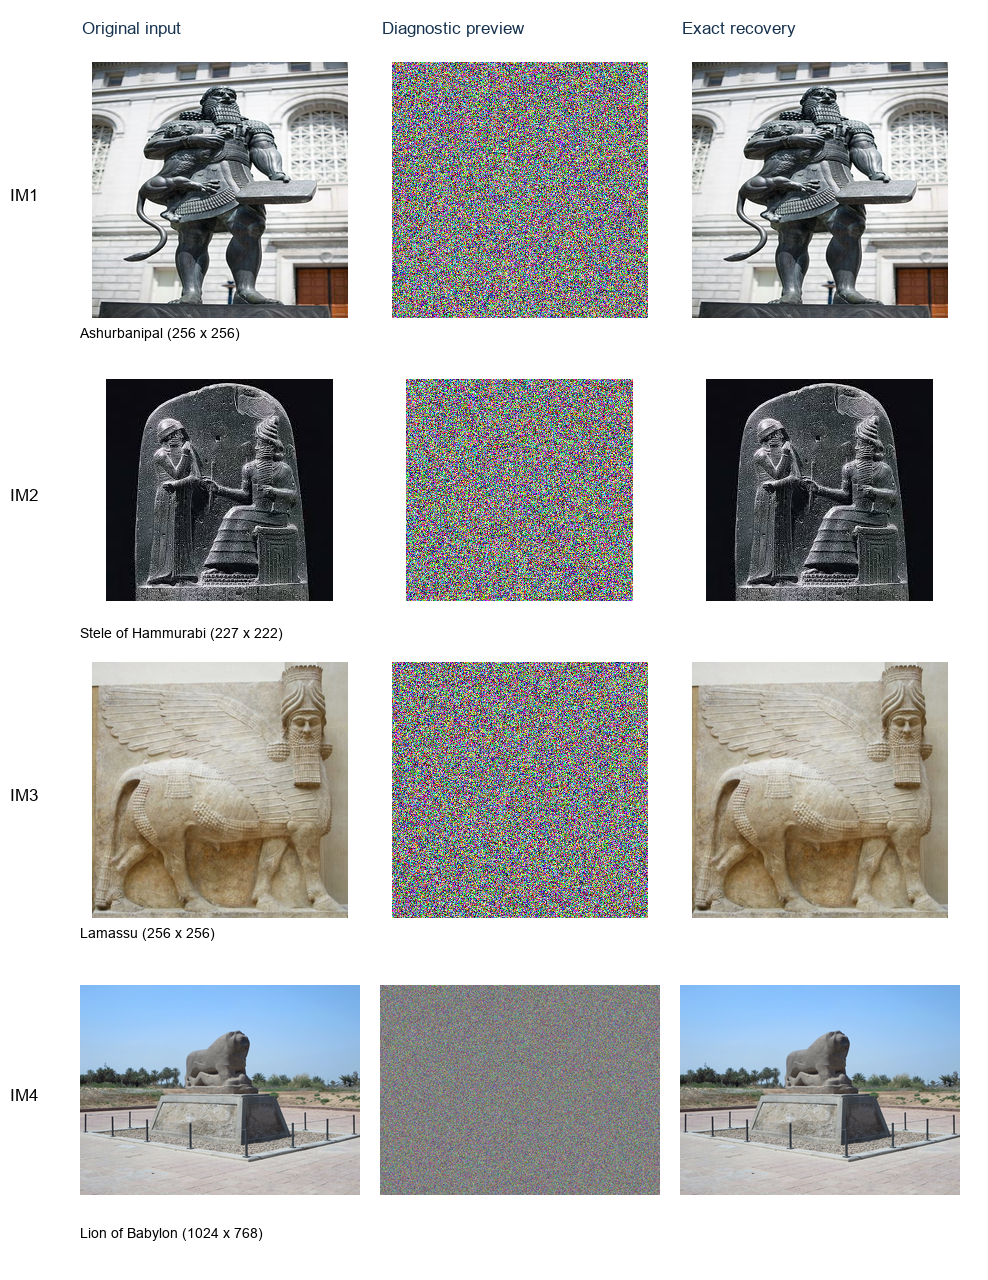
\includegraphics[width=\linewidth,height=0.82\textheight,keepaspectratio]{figures/native_panel.png}
\end{center}
\small Source, diagnostic preview, and exact recovery. These inspection previews are not the quantum ciphertext furnished to an adversary in the theorem.

\newpage
\section*{11. \(256\times256\) visual verification}
\begin{center}
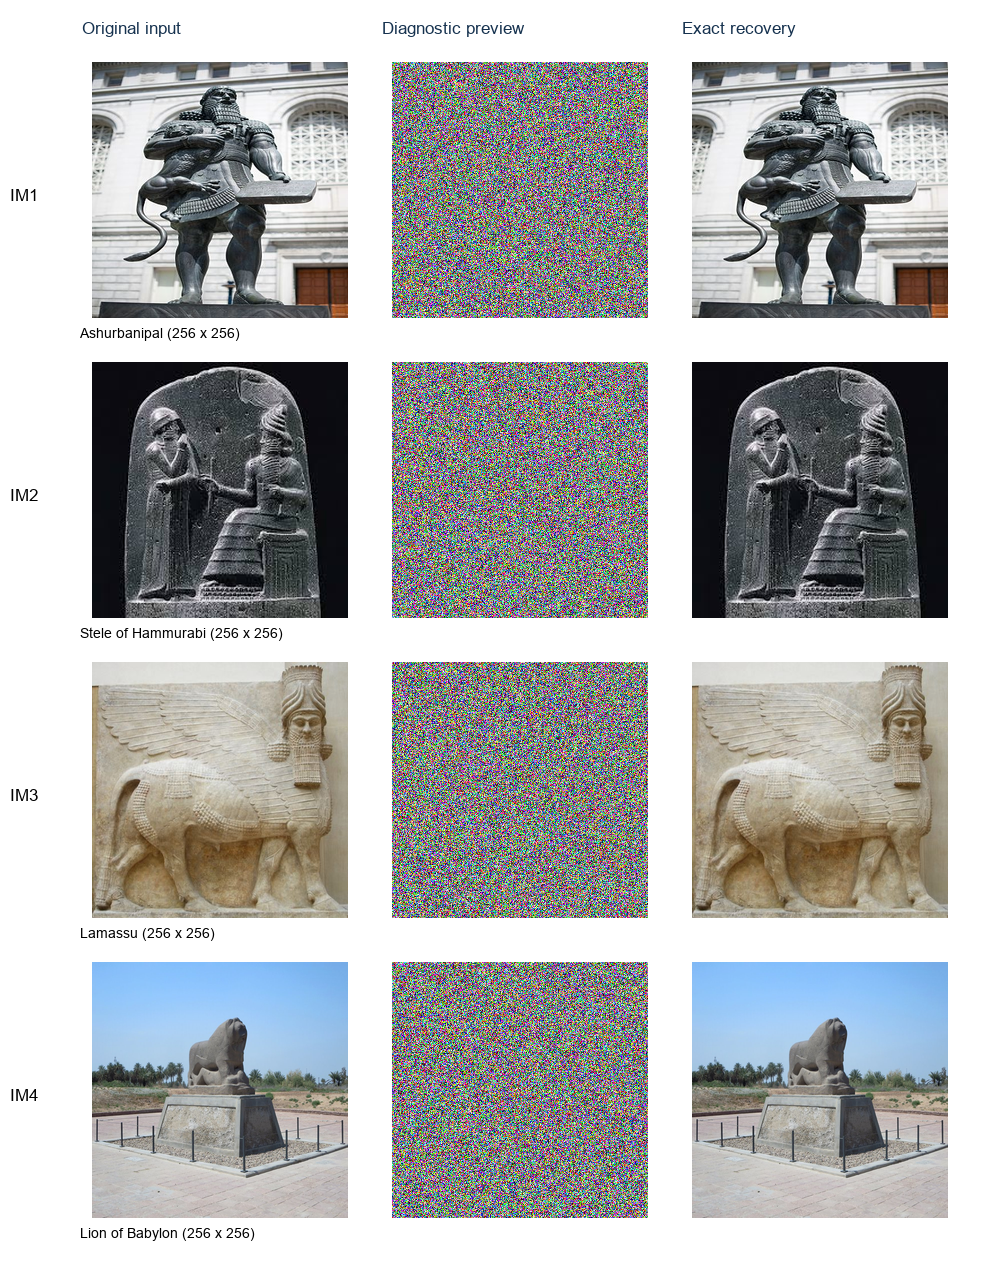
\includegraphics[width=\linewidth,height=0.82\textheight,keepaspectratio]{figures/paper256_panel.png}
\end{center}
\small The same four source images, using the explicitly specified resize profile. All recovered RGB bytes match that profile exactly.

\newpage
\section*{12. All 24 runs and practical scope}
\begin{center}
{\footnotesize
\setlength{\tabcolsep}{4pt}
\begin{tabular}{@{}lrrrrr@{}}
\toprule
Run & $N$ & Enc. s & Dec. s & $|1-F|$ & Max norm error \\
\midrule
native\_IM1\_r1 & 65,536 & 1.444 & 1.473 & $1.55\times10^{-15}$ & $3.77\times10^{-15}$ \\
native\_IM1\_r2 & 65,536 & 1.402 & 1.438 & $1.55\times10^{-15}$ & $3.55\times10^{-15}$ \\
native\_IM1\_r3 & 65,536 & 1.431 & 1.480 & $1.33\times10^{-15}$ & $3.66\times10^{-15}$ \\
native\_IM2\_r1 & 50,394 & 1.062 & 1.099 & $2.00\times10^{-15}$ & $3.77\times10^{-15}$ \\
native\_IM2\_r2 & 50,394 & 1.048 & 1.069 & $2.00\times10^{-15}$ & $3.55\times10^{-15}$ \\
native\_IM2\_r3 & 50,394 & 1.048 & 1.073 & $2.00\times10^{-15}$ & $4.11\times10^{-15}$ \\
native\_IM3\_r1 & 65,536 & 1.390 & 1.418 & $1.55\times10^{-15}$ & $3.66\times10^{-15}$ \\
native\_IM3\_r2 & 65,536 & 1.382 & 1.412 & $1.33\times10^{-15}$ & $3.89\times10^{-15}$ \\
native\_IM3\_r3 & 65,536 & 1.379 & 1.412 & $1.55\times10^{-15}$ & $4.22\times10^{-15}$ \\
native\_IM4\_r1 & 786,432 & 16.620 & 16.957 & $4.44\times10^{-16}$ & $4.00\times10^{-15}$ \\
native\_IM4\_r2 & 786,432 & 15.276 & 15.648 & $4.44\times10^{-16}$ & $3.89\times10^{-15}$ \\
native\_IM4\_r3 & 786,432 & 14.727 & 15.032 & $4.44\times10^{-16}$ & $4.00\times10^{-15}$ \\
paper256\_IM1\_r1 & 65,536 & 1.232 & 1.266 & $1.55\times10^{-15}$ & $3.66\times10^{-15}$ \\
paper256\_IM1\_r2 & 65,536 & 1.238 & 1.241 & $1.33\times10^{-15}$ & $3.89\times10^{-15}$ \\
paper256\_IM1\_r3 & 65,536 & 1.251 & 1.269 & $1.55\times10^{-15}$ & $3.77\times10^{-15}$ \\
paper256\_IM2\_r1 & 65,536 & 1.233 & 1.276 & $1.33\times10^{-15}$ & $3.89\times10^{-15}$ \\
paper256\_IM2\_r2 & 65,536 & 1.221 & 1.247 & $1.55\times10^{-15}$ & $3.66\times10^{-15}$ \\
paper256\_IM2\_r3 & 65,536 & 1.240 & 1.264 & $1.33\times10^{-15}$ & $3.89\times10^{-15}$ \\
paper256\_IM3\_r1 & 65,536 & 1.241 & 1.266 & $1.55\times10^{-15}$ & $3.66\times10^{-15}$ \\
paper256\_IM3\_r2 & 65,536 & 1.231 & 1.245 & $1.55\times10^{-15}$ & $3.77\times10^{-15}$ \\
paper256\_IM3\_r3 & 65,536 & 1.218 & 1.253 & $1.33\times10^{-15}$ & $3.66\times10^{-15}$ \\
paper256\_IM4\_r1 & 65,536 & 1.228 & 1.255 & $1.33\times10^{-15}$ & $3.89\times10^{-15}$ \\
paper256\_IM4\_r2 & 65,536 & 1.209 & 1.236 & $1.33\times10^{-15}$ & $3.66\times10^{-15}$ \\
paper256\_IM4\_r3 & 65,536 & 1.234 & 1.237 & $1.33\times10^{-15}$ & $3.44\times10^{-15}$ \\
\bottomrule
\end{tabular}}
\end{center}


Times are local classical-simulator seconds. The \(3Nr\) base rotations are position-controlled operations; they must not be counted as ordinary uncontrolled one-qubit gates when estimating physical hardware cost. This package verifies the logical operator and exact factorization, not a transpiled large-image IBM circuit.

No physical noise correction or active-attack authentication is inferred. The final privacy formula is for the v2 key law and fresh-key quantum-state interface defined on pages 1--4.

\newpage
\section*{13. Reproduction and manuscript-ready statement}
The requested delivery folder contains the implementation, exact original input files, 24 private research key records, all tables, numerical evidence, and this analysis. The private key folder must be excluded from a public research supplement.

Run \texttt{REPRODUCE.ps1} to replay the saved private simulation keys, or the documented Python commands. Replay is an offline reproducibility mode, not a protocol allowing key reuse in transmission.

A physical QRNG may replace the reference key provider only with an appropriate uniformity/extraction guarantee. A deterministic HCS unitary mixing function can replace \(W_k\) if independent of the reserved privacy core; the proof does not require a chaos assumption.

\textbf{Proposed revised security statement:}
{\color{red}
For the corrected QIRBP instantiation, encryption is implemented as a position-controlled substitution containing fresh uniform feature Pauli masks and position phases, followed by a reversible affine address permutation with an exactly uniform secret offset and a position-controlled CNOT/CZ layer. Averaging over the independent privacy core gives a replacement channel on the valid input subspace, including arbitrary reference systems. Hence its ideal one-use distinguishing advantage is zero. With fresh independent keys on every encryption call, the same conclusion holds for a sequence of valid-input calls. This is a guarantee for the specified corrected key law; generic tomography complexity and nominal Grover search estimates are not interpreted as attack lower bounds. Large-image experiments reported here are exact local simulations, and diagnostic PNG inspection statistics are separated from the quantum-state security guarantee.
}

\begin{thebibliography}{9}
\bibitem{private}
M. Mosca, A. Tapp, R. de Wolf, \emph{Private Quantum Channels and the Cost of Randomizing Quantum Information}.
\url{https://arxiv.org/abs/quant-ph/0003101}.
\bibitem{watrous}
J. Watrous, \emph{The Theory of Quantum Information}, Chapter 3: discrimination and trace-norm contractivity.
\url{https://cs.uwaterloo.ca/~watrous/TQI/TQI.3.pdf}.
\bibitem{secrets}
Python Software Foundation, \emph{secrets: Generate secure random numbers for managing secrets}.
\url{https://docs.python.org/3/library/secrets.html}.
\bibitem{qirbp}
N. A. Alwan et al., \emph{A multi-channel quantum image representation model with qubit sequences for quantum-inspired image and image retrieval}, AIMS Mathematics 10(5), 10994--11035 (2025).
\url{https://doi.org/10.3934/math.2025499}.
\end{thebibliography}
\end{document}
